\documentclass[aspectratio=169,11pt]{beamer}
\usepackage{graphicx,booktabs,amsmath}
\definecolor{navy}{HTML}{19344C}\definecolor{blue}{HTML}{255795}\definecolor{rust}{HTML}{A94520}
\setbeamertemplate{navigation symbols}{}
\setbeamercolor{normal text}{fg=navy,bg=white}
\setbeamercolor{frametitle}{fg=navy}
\setbeamerfont{frametitle}{series=\bfseries,size=\Large}
\setbeamercolor{structure}{fg=blue}
\setbeamersize{text margin left=9mm,text margin right=9mm}
\setbeamertemplate{footline}{\hfill\textcolor{navy}{\scriptsize COSI 126A \hspace{5mm} \insertframenumber\hspace{8mm}}\vskip3mm}
\newcommand{\key}[1]{{\color{blue}\bfseries #1}}
\newcommand{\notefoot}[1]{\par\vfill{\scriptsize\color{navy}#1}}
\hypersetup{pdftitle={Selective Reconstruction in IDEC},pdfauthor={John Zhang and Ryan Jian}}
\begin{document}
\begin{frame}
\vfill
{\small\color{rust}Unsupervised Learning and Data Mining}\par\vspace{5mm}
{\fontsize{30}{34}\selectfont\bfseries Selective reconstruction in IDEC}\par\vspace{3mm}
{\Large Digit clustering with an adaptive Gaussian\\and image-specific saliency}\par\vspace{8mm}
{\normalsize\bfseries John Zhang and Ryan Jian}
\vfill
\end{frame}

\begin{frame}{Why IDEC keeps a decoder}
\key{Original research question}\par
Guo et al.\ investigate whether preserving local structure improves joint learning of an embedding and its clusters.\par\bigskip
\begin{columns}[T,onlytextwidth]
\column{.47\textwidth}
\key{Challenge}\par\smallskip
DEC learns from its own assignments. Reinforcing an early error can separate similar inputs.
\column{.48\textwidth}
\key{Philosophy and solution}\par\smallskip
Keep enough information in the code to reconstruct each input. IDEC adds pixel reconstruction error to DEC's clustering loss.
\end{columns}
\vfill
\key{Paper reproduction}\quad 88.06\% published $\;\cdot\;$ 88.10\% reproduced\par
{\small All 70,000 MNIST digits used for fitting and scoring with author-pretrained weights.}
\notefoot{\href{https://www.ijcai.org/proceedings/2017/243}{Guo et al., IJCAI 2017}\quad $\cdot$\quad \href{https://proceedings.mlr.press/v48/xieb16.html}{Xie et al., ICML 2016}}
\end{frame}

\begin{frame}{A background change with the handwriting held fixed}
\begin{columns}[c,onlytextwidth]
\column{.51\textwidth}
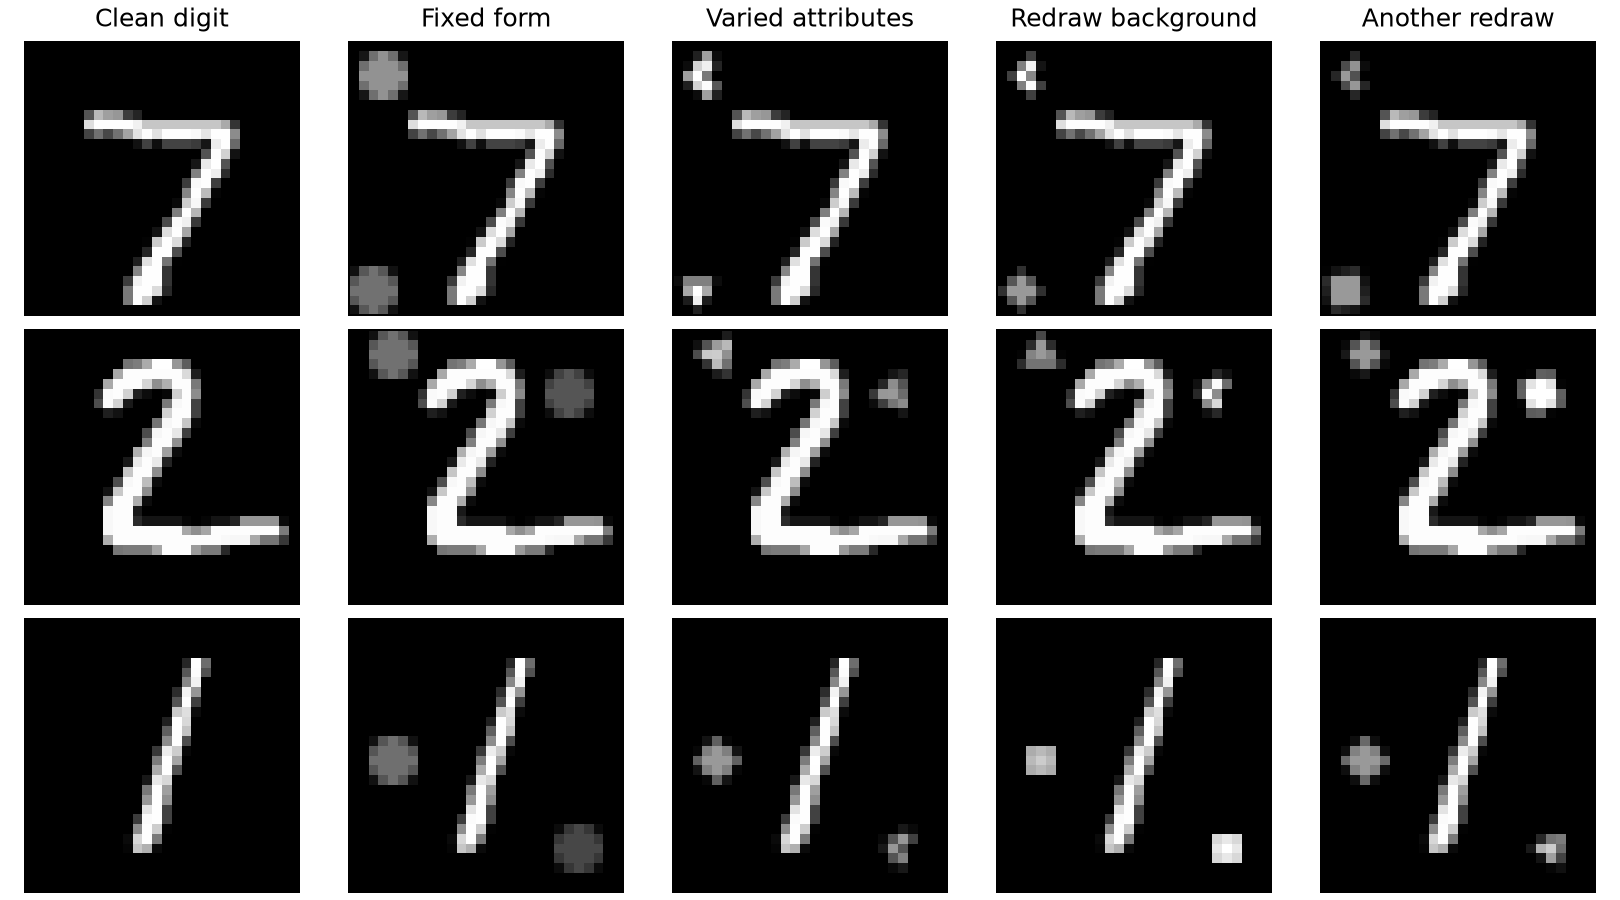
\includegraphics[width=\linewidth]{../figures/varied.png}
\column{.45\textwidth}
\key{Our research question}\par\smallskip
We test whether the reward for reconstructing irrelevant features harms digit clustering.\par\medskip
Two small symbols occupy blank space. Changing their shape, angle, brightness or size leaves every stroke intact.
\end{columns}
\notefoot{The marks test a known nuisance. The primary model learns from clean digits alone.}
\end{frame}

\begin{frame}{The reconstruction target affects digit accuracy}
\begin{columns}[T,onlytextwidth]
\column{.46\textwidth}
\key{Does the background hurt?}\par\smallskip
Matched-domain fits, clean versus marked\par\medskip
\begin{tabular}{lrr}\toprule &Clean&Marked\\\midrule
DEC &77.63&70.86\\
IDEC &73.23&65.14\\\bottomrule
\end{tabular}\par\medskip
Both decline in all five seeds. IDEC loses 1.32 points more on average.
\column{.49\textwidth}
\key{Does copying the background matter?}\par\smallskip
Same marked inputs, different decoder targets\par\medskip
\begin{tabular}{lr}\toprule Target in both stages&ACC\\\midrule
Marked image&65.40\\
Known clean digit&71.44\\\bottomrule
\end{tabular}\par\medskip
Changing only the target gains \key{6.04 points}, positive in all five seeds.
\end{columns}
\notefoot{Values are accuracy (\%). The right panel is a separate experiment. Its clean target is available from the generator.}
\end{frame}

\begin{frame}{Which reconstruction errors should count more?}
\key{Our philosophy}\par
Use two clues available without labels to give likely digit strokes more weight.\par\medskip
\begin{columns}[T,onlytextwidth]
\column{.48\textwidth}
\key{Adaptive Gaussian}\par\smallskip
Start with a broad Gaussian at image center. Use its intensity-weighted centroid to locate a new Gaussian for this image.
\column{.47\textwidth}
\key{Cluster saliency}\par\smallskip
A frozen autoencoder and K-means teacher identify pixels that influence the distance gap between its two closest clusters.
\end{columns}
\medskip
\[
 w_x(p)\ \propto\ G(p;c_x)\,[0.5+S_x(p)] \qquad
 L_{\rm pre}=\mathrm{mean}_p\big[w_x(p)(x_p-\hat x_p)^2\big]
\]
Normalize weights to mean one per image. Apply them in pretraining, then fine-tune with ordinary IDEC.
\end{frame}

\begin{frame}{What the student is rewarded for reconstructing}
\centering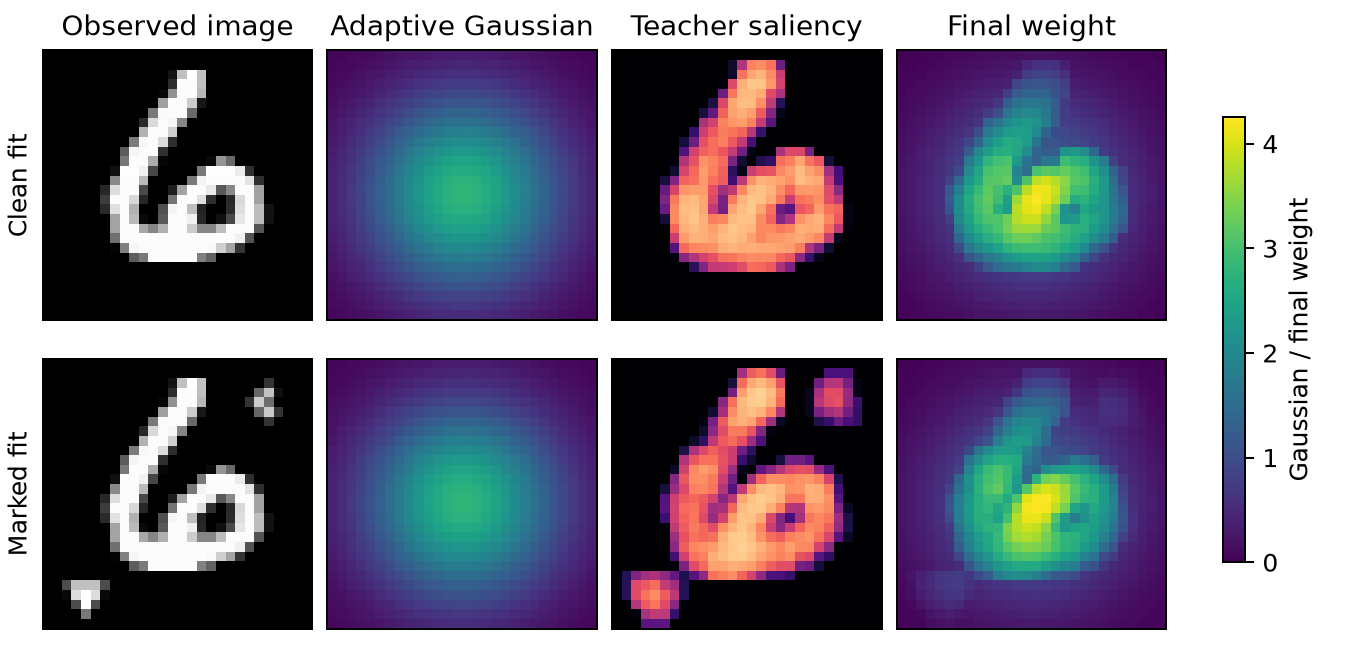
\includegraphics[height=.59\paperheight]{../final/weights.png}\par
\small Same handwriting, two training domains. Marked-fit weights average \key{2.62 on digit ink} and \key{0.91 on the symbols}. Uniform loss gives both a weight of one.
\end{frame}

\begin{frame}{The main test introduces symbols after training}
\begin{enumerate}
\item Fit the teacher and student on \key{12,000 clean, unlabeled digits}. All methods use the same split and five student seeds.
\item Freeze the student. Score the \key{same 10,000 held-out digits} first clean, then with two background symbols.
\item Compare uniform loss, each component alone and their products. Shuffle saliency maps to test whether matching the map to its own image matters.
\end{enumerate}
\vfill
{\small Digit labels are used after training to score clusters. A separate marked-training experiment measures performance when symbols are present during fitting.}
\end{frame}

\begin{frame}{The combined weights gain 6.98 points over IDEC}
\centering\small
\begin{tabular}{lrrr}
\toprule
& \multicolumn{2}{c}{Clean fit} & Marked fit\\
\cmidrule(lr){2-3}Pretraining weights & Clean test & Marked test & Marked test\\\midrule
Ordinary IDEC & 73.23 & 64.62 & 65.14\\
Fixed Gaussian & 74.07 & 68.92 & 68.80\\
Saliency only & 71.83 & 64.33 & 67.51\\
Adaptive Gaussian & 76.20 & 70.28 & 69.71\\
Fixed Gaussian $\times$ saliency & 75.95 & 71.51 & 70.52\\
Adaptive $\times$ shuffled saliency & 73.80 & 68.47 & 68.63\\
\midrule
\textbf{Adaptive $\times$ aligned saliency} & \textbf{76.10} & \textbf{71.59} & \textbf{71.06}\\
\bottomrule
\end{tabular}
\par\medskip
\raggedright
\key{Primary endpoint}\quad After clean training, the final model reaches 71.59\% on marked digits, up from 64.62\% in ordinary IDEC. Every paired seed improves.
\notefoot{All table entries are mean digit accuracy (\%) across the same five student seeds.}
\end{frame}

\begin{frame}{How much does moving the center add?}
\centering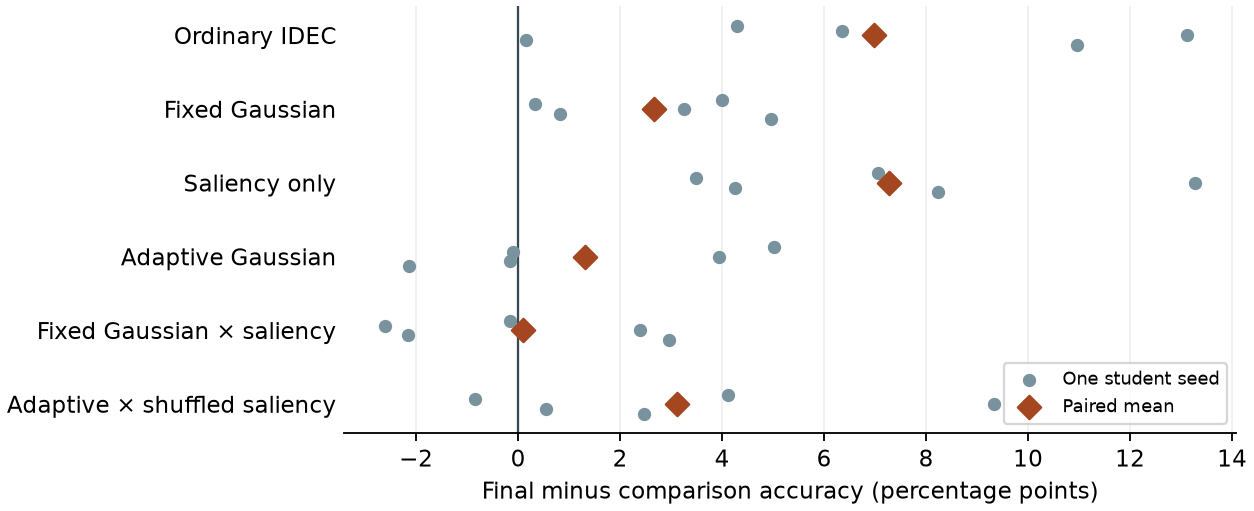
\includegraphics[height=.52\paperheight]{../final/paired.png}\par
\raggedright\small
With the same saliency, moving the center adds \key{0.09 points} on average (two of five seeds improve). With the same adaptive center, aligning saliency to the image gains \key{3.12 points} over shuffling it (four of five improve).
\end{frame}

\begin{frame}{What the experiment establishes}
\key{Drawback}\par
On identical marked inputs, a decoder trained to recover only the digit yields better clusters. The reconstruction target contributes to the performance loss.\par\medskip
\key{Solution}\par
Adaptive Gaussian $\times$ image-specific saliency narrows the clean-trained model's accuracy loss from \textbf{8.62 to 4.50 points} when marks appear.\par\medskip
\key{Boundary}\par
A fixed Gaussian with aligned saliency performs almost identically. DEC reaches 75.62\% on the same primary test. A central distractor or an off-center digit could violate the spatial assumption.
\notefoot{\href{https://github.com/JohnR31N/cs126FinalProj/tree/idec-final-v2.0}{Public code, per-image assignments, report and reproduction commands}}
\end{frame}
\end{document}
